
Każda zakładka z obrazem lub obrazami jest implementowana przez klasę \sokarclass{DicomView}.

Interfejs graficzny \sokarclass{DicomView} posiada następujące elementy:
\begin{itemize}
    \item pasek narzędzi znajdujący się na górze - implementowany za pomocą klasy \sokarclass{DicomToolBar}, opisany w sekcji \ref{sec:sokar-dicomtoolbar}
    \item miejsce na scene z obrazem DICOM na środku - implementowany za pomocą klasy \sokarclass{DicomGraphics}, opisany w sekcji \ref{sec:sokar-dicomgraphics}
    \item suwak filmu w dolnej części - implementowany za pomocą klasy \sokarclass{MovieBar}, opisany w sekcji \ref{sec:sokar-moviebar}
    \item podgląd miniaturek obrazów w prawej części - implementowany za pomocą klasy \sokarclass{FrameChooser}, opisany w sekcji \ref{sec:sokar-framechooser}
\end{itemize}

Dodatkowo posiada obiekt \sokarclass{DicomSceneSet}, który jest zbiorem obrazów opisany w sekcji \ref{sec:sokar-scenesets}.
\sokarclass{DicomView} łączy zdarzenia wysyłane przez wszystkie obiekty.

Poniżej jest opisane zachowanie tych elementów:

\subsection{Elementy interfejsu graficznego}

\begin{figure}[!htbp]
    \centering
    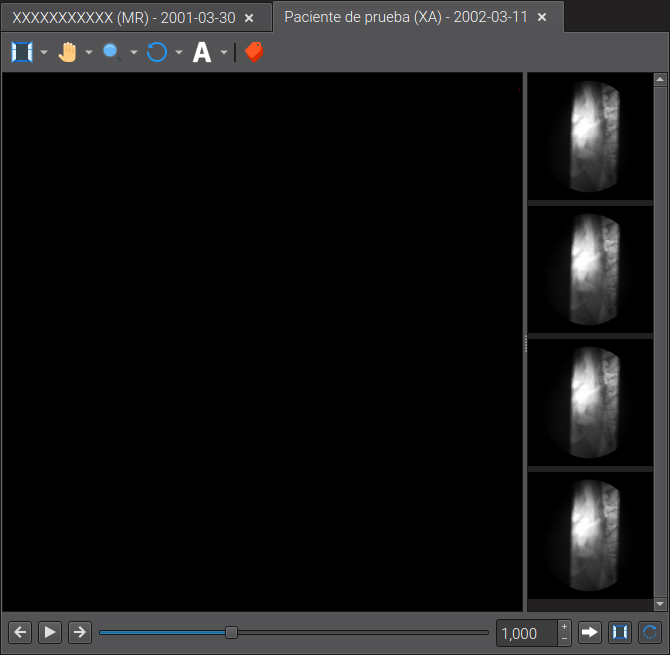
\includegraphics[width=\textwidth]{img/sokar-dicomview-001.png}
    \caption{Wygląd DicomView}
    \label{fig:sokar-dicomview001}
\end{figure}

\subsubsection{\sokarclass{DicomToolBar}}
\label{sec:sokar-dicomtoolbar}

Jest to pasek narzędzi znajdujący się na górze \sokarclass{DicomView}.
Posiada on zespół ikonek z rozwijalnymi menu kontekstowymi.
Kliknięcie odpowiedniej ikony spowoduje wysłanie sygnału do obecnie wyświetlanej sceny.

Są dwa sygnału Qt wysyłane przez klase:
\begin{itemize}
    \item \cppcode{void stateToggleSignal(State state);}

          Sygnał ten oznacza zmianę stanu interfejsu

    \item \cppcode{void actionTriggerSignal(Action action, bool state = false);}
\end{itemize}


Ikony na pasku:
\begin{itemize}
    \item Okienkowanie
    \item Przesuwanie
    \item Skalowanie
    \item Rotacja
    \item Indicators
    \item Tagi - czerwona ikonka dwóch metek

          Kliknięcie
\end{itemize}

\subsubsection{\sokarclass{DicomGraphics}}
\label{sec:sokar-dicomgraphics}

\subsubsection{\sokarclass{MovieBar}}
\label{sec:sokar-moviebar}

\par
Jest paskiem filmu w dolnej części \sokarclass{DicomView}.
Element graficzny ma dostęp do sekwencji scen i ukrywa swoją obecność przed użytkownikiem, kiedy w sekwencji jest tylko jedna scena.

\par
Pasek jest podzielony na trzy części: trzy przyciski znajdujące się po lewej, pasek pokazujący postępu sekwencji na środku i prządka z trzema przyciskami po prawej.

\par
Trzy lewe przyciski odpowiadają za poruszanie się po sekwencji.
Wciśniecie pierwszego przycisku (XXX) powoduje zatrzymanie upływu sekwencji i wysłanie sygnału \sokarfunction{SceneSequence}{stepBackward} do sekwencji.
Wciśniecie drugiego przycisku (XXX) powoduje włączenie lub wyłączenie upływu sekwencji.
Wciśniecie trzeciego przycisku (XXX) powoduje zatrzymanie upływu sekwencji i wysłanie sygnału \sokarfunction{SceneSequence}{stepForward} do sekwencji.
\par
Pasek (XXX) pokazujący postępu sekwencji jest obiektem klasy \qtclass{QSlider}.
Odświeżanie paska jest wrażliwe na sygnał \sokarfunction{SceneSequence}{steped} of sekwencji.
\par
Elementy po prawej stronie definiuje parametry trybu filmowego.
Prządka, element do wprowadzania liczby zmiennoprzecinkowej klasy \qtclass{QDoubleSpinBox}.
Im większa wartość liczby tym klatki filmu są dłużej wyświetlane.
Drugi przycisk pozwala zmienić sposób przemiatania.
Trzeci przycisk wymusza tryb jednego okna dla wszystkich klatek filmu.
Jeżeli mamy załadowanych wile obrazów tego samego badania, to nie koniecznie muszą mieć to samo okno.
Dodatkowo ten tryb pozwala wprowadzić jednolite okienko dla wszystkich klatek po zmianie parametrów tego okienka na jednej klatce.
Czwarty i ostatni przycisk służy do użycia jednej macierzy transformaty na wszystkich klatkach.

\paragraph*{Tryb filmowy}

\par
Tryb filmowy można aktywować jedynie wtedy gdy w sekwencji scen jest więcej niż jedna scena.
Włączenie trybu filmowego polega na stworzeniu obiektu klasy \sokarclass{MovieMode}.
Obiekt ten zapisuje wskaźnik go obecnie wyświetlanej sceny, to czy powinno być użyte to samo okno, oraz to czy powinna być używana ta sama transformata.
Następnie obiekt ten jest wysyłany do wszystkich scen w sekwencji.
Uruchamiany jest timer, obiekt klasy \qtclass{QTimer}, na czas równy czasu trwania sceny zapisanego w kroku przemnożonego przez liczbę z prządki.
Po upływie timera, wstawiana jest nowa scena za pomocą sygnały \sokarfunction{MovieBar}{setStep}, a timer jest ustawiany nan nowo.

\subsubsection{\sokarclass{FrameChooser}}
\label{sec:sokar-framechooser}

Ten element to wybór scen za pomocą ikon, implementowany przez klasę \sokarclass{DicomView}.
Element, podobnie jak pasek filmu ma dostęp do sekwencji scen i ukrywa swoją obecność przed użytkownikiem, kiedy w sekwencji jest tylko jedna scena.
Po wciśnięciu ikony jest zmieniana scena.